\chapter{SIMPLIFIED EXPLANATION OF THE PROPOSED CONTROL SCHEME}
In a current controlled inverter or DSTATCOM, the inverter/compensator current is regulated based on the voltage of its filter inductor. Referring to Fig.\,\ref{fig4.1}, the voltage across filter inductor in phase-$a$ is given as below.
\begin{equation}
v_{Lsha} = L_{sh}\frac{di_{sha}}{dt} = (v_{ao} - v_{No}) - v_{ga}
\end{equation}
This clearly indicates that in order to achieve a positive slope of the compensator current, the inductor voltage should be positive, and vice versa. It can also be concluded that the sign of inductor voltage is changed by controlling the term $(v_{ao} - v_{No})$. From \eqref{4.2}, it can be stated that the voltage $v_{No}$ depends on all the pole voltages $v_{ao}, \, v_{bo}, \, v_{co}$, and $v_{fo}$. The pole voltages have a value of $+\frac{v_{dc}}{2}$ when the corresponding top switch of the leg is turned ON, and $-\frac{v_{dc}}{2}$ when the top switch is turned OFF. Therefore, it is not possible to control the switches on the phase-$a$ leg alone to change the sign of the inductor voltage, since $(v_{ao} - v_{No})$ depends on all switch states. This is due to the presence of $v_{No}$. By transforming the above equation to the $dq$ frame, the $dq$ equivalent of $v_{No}$ does not exist, and thus the sign of the inductor voltage in the $dq$ frame is controlled by the $dq$ equivalent of $v_{ao}$. Hence, it becomes straightforward to generate switching pulses for the switches in phase-$a$ leg and similarly in other legs. 

\begin{figure}[]\centering
	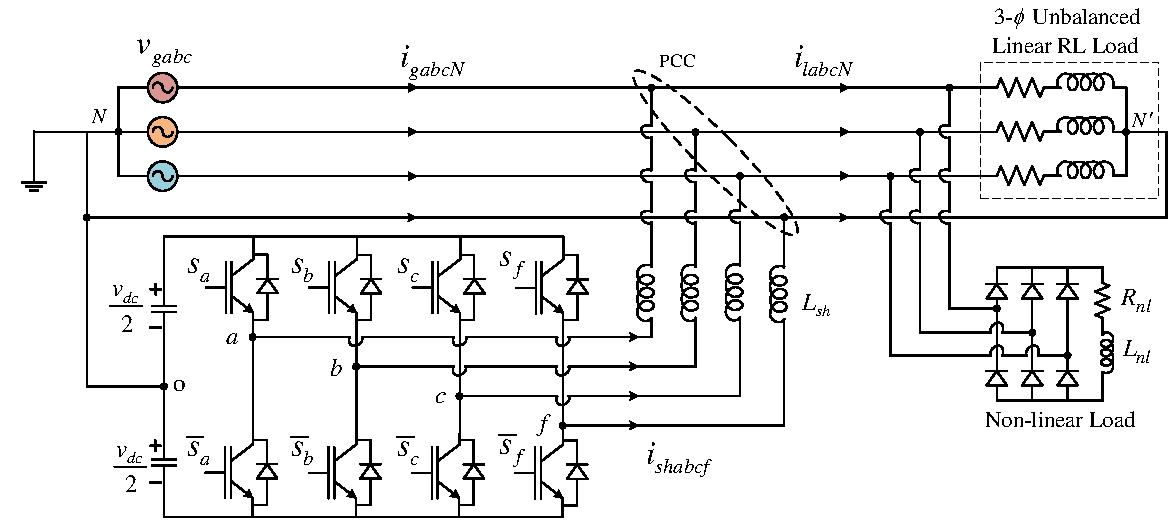
\includegraphics[scale=0.72	]{figures/Appendix/4leg_DSTATCOM1.pdf}
	\caption{\small Equivalent schematic diagram of a four-leg voltage source converter based DSTATCOM} %\vspace*{-0.4cm}
	\label{A1.fig1}
\end{figure} 
However, if the circuit diagram of DSTATCOM system is redrawn while preserving its dynamics, as shown in Fig.\,\ref{A1.fig1}, the selection of switching pulses would become simpler. In this figure, the neutral-point voltage (NPV), $v_{No}$ is represented based on the expression given in \eqref{4.4}, i.e., $v_{No} = L_{sh} \frac{0.25i_{sh\gamma}}{dt}.$ From the Fig.\,\ref{A1.fig1}, the voltage across filter inductor in phase-$a$ is given as below.
\begin{equation}
v^\prime_{Lsha} = L_{sh}\frac{d}{dt}\Big\{ i_{sha} + 0.25 i_{sh\gamma} \Big\} = v_{ao} - v_{ga}
\end{equation}
This clearly indicates that the sign of inductor voltage is changed by controlling $v_{ao}$ alone. Therefore, to achieve a positive sign of inductor voltage, the top switch of the respective leg, in this case the phase-$a$ leg, should be turned ON. This action sets the pole voltage $v_{ao}$ to $+\frac{v_{dc}}{2}$. Similarly, to obtain a negative sign of inductor voltage, the top switch should be turned OFF. 
In summary, by controlling ($i_{sha} + 0.25 i_{sh\gamma}$) instead of $i_{sha}$ alone, the selection of switching pulses becomes easier. Thus, the sliding surface is proposed as $\sigma_{a} = (i_{sha}+0.25i_{sh\gamma}) - (i^{*}_{sha}+0.25i^{*}_{sh\gamma})$ for the DSTATCOM system. 

The similar analysis is carried out for the DVR system shown in Fig.\,\ref{fig5.1}. In a voltage controlled inverter or DVR, the inverter/compensator voltage is controlled by the voltage across its filter capacitor. The capacitor voltage is controlled by its current, which is determined by the voltage across the filter inductor. The inductor voltage is, in turn, controlled by the state of switches. Referring to Fig.\,\ref{fig5.1}, the voltage across the filter inductor in phase-$a$ is given as below.
\begin{equation}
\begin{aligned}
v_{L1a} &= L_{1}\frac{di_{1a}}{dt} = (v_{ao} - v_{f^\prime o}) - v_{ca} \\
        &= L_{1}\frac{d}{dt} \Big\{i_{ca} + i_{l^{\prime}a} \Big\} = (v_{ao} - v_{f^\prime o}) - v_{ca} \\
        &= L_{1}\frac{di_{ca}}{dt} = (v_{ao} - v_{f^\prime o}) - v_{ca} - \frac{L_1}{L_t} \Big\{ v_{ca} + v_{Da} \Big\} \\
        &= L_{1}C_f\frac{d^2v_{ca}}{dt^2} = (v_{ao} - v_{f^\prime o}) - \Big\{ 1 + \frac{L_1}{L_t} \Big\} v_{ca} -  \frac{L_1}{L_t} v_{Da}  
\end{aligned}
\end{equation}
This equation indicates that to have a positive slope of inductor current, the inductor voltage should be positive and vice versa.  It also implies that the sign of the inductor voltage can be changed by controlling $(v_{ao} - v_{f^\prime o})$ while keeping $v_{ca}$ and $v_{Da}$ known. From \eqref{5.2}, it can be stated that the voltage $v_{f^\prime o}$ depends on all the pole voltages $v_{ao}, \, v_{bo}, \, v_{co}$, and $v_{fo}$. The pole voltages have a value of $+\frac{v_{dc}}{2}$ when the corresponding top switch of the leg is turned ON and $-\frac{v_{dc}}{2}$ when the top switch is turned OFF. Therefore, controlling the switches on the phase-$a$ leg alone cannot change the sign of the inductor voltage since  $(v_{ao} - v_{f^\prime o})$ depends on all the states of switches. 

\begin{figure}[]\centering
	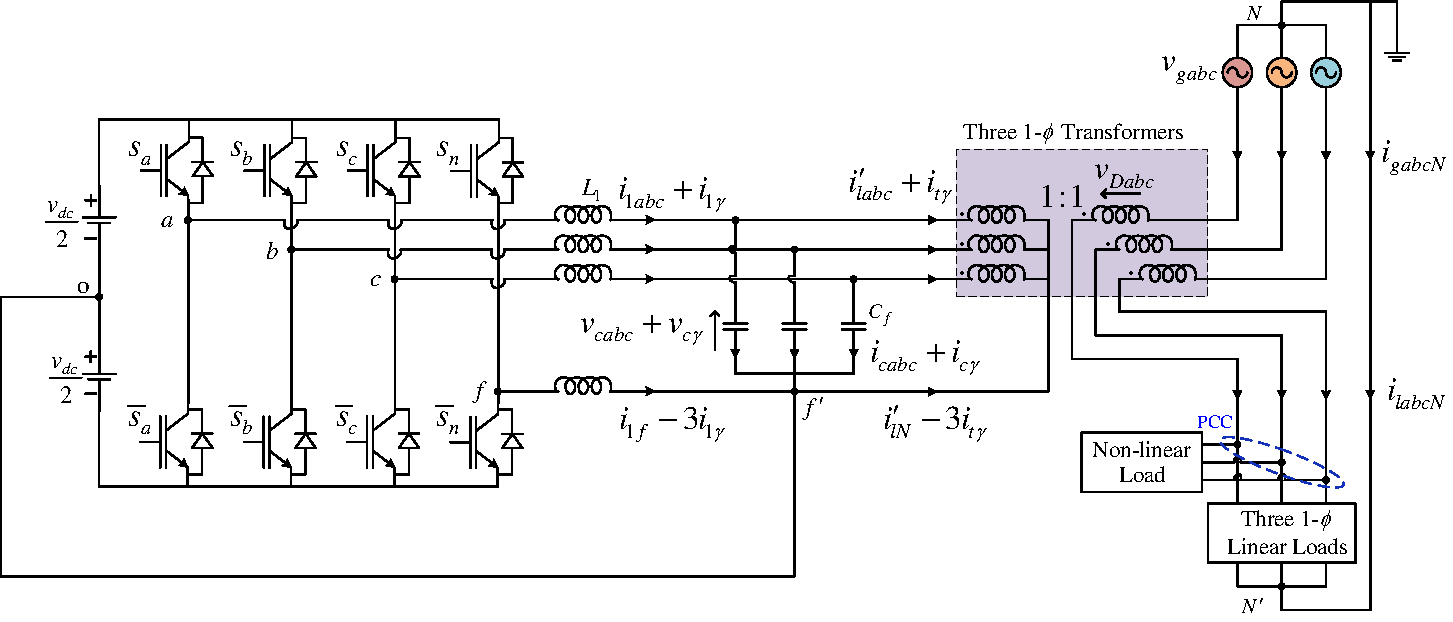
\includegraphics[scale=0.6	]{figures/Appendix/4leg_DVR1.pdf}
	\caption{\small Equivalent schematic diagram of a four-leg voltage source converter based DVR} %\vspace*{-0.4cm}
	\label{A1.fig2}
\end{figure} 
If the circuit diagram of DVR system is redrawn while preserving its dynamics as shown in Fig.\,\ref{A1.fig2}, the selection of switching pulses would become simpler. In this modified figure, the neutral-point voltage (NPV), $v_{f^\prime o}$ is represented based on the expression given in \eqref{5.4}. From the Fig.\,\ref{A1.fig2}, the voltage across filter inductor in phase-$a$ is given as below.
\begin{equation}
\begin{aligned}
v^\prime_{L1a} &= L_{1}\frac{d}{dt} \Big\{i_{1a} + i_{1\gamma} \Big\} = v_{ao}  - (v_{ca} + v_{c\gamma}) \\
               &= L_{1}\frac{d}{dt} \Big\{i_{ca} + i_{c\gamma} + i_{l^{\prime}a} + i_{t\gamma} \Big\}  = v_{ao}  - (v_{ca} + v_{c\gamma}) \\
&= L_{1}\frac{d}{dt} \Big\{ i_{ca} + i_{c\gamma} \Big\} = v_{ao}  - (v_{ca} + v_{c\gamma}) - \frac{L_1}{L_t} \Big\{ v_{ca} + v_{c\gamma} + v_{Da} \Big\} \\
&= L_{1}C_f\frac{d^2}{dt^2} \Big\{ v_{ca} + v_{c\gamma} \Big\} = v_{ao} - \Big\{ 1 + \frac{L_1}{L_t} \Big\} (v_{ca} + v_{c\gamma}) -  \frac{L_1}{L_t} v_{Da}  
\end{aligned}
\end{equation}
This equation reveals that the sign of inductor voltage or the sign of the slope of $v_{ca} + v_{c\gamma}$ can be changed by controlling $v_{ao}$ alone. Therefore, to obtain a positive sign of inductor voltage or a positive slope of $v_{ca} + v_{c\gamma}$, the top switch of respective leg (in this case, phase-$a$ leg) should be turned ON. This action sets the pole voltage $v_{ao}$ to $+\frac{v_{dc}}{2}$. Similarly, to achieve a negative sign of inductor voltage or negative slope of $v_{ca} + v_{c\gamma}$, the top switch should be turned OFF.
In summary, by controlling ($v_{ca} + v_{c\gamma}$) instead of $v_{ca}$ alone, the selection of switching pulses becomes easier. Therefore, the proposed sliding surface for the DVR system is $\sigma_{a} = \Big(\lambda_a + \frac{d}{dt}\Big) x_a$, where $x_a = (v_{ca} + v_{c\gamma}) - (v^*_{ca} + v^*_{c\gamma})$. 